\section{Управление рисками предприятия, методы оценки рисков}

Управление рисками --- это процессы, связанные с идентификацией, анализом рисков и принятием решений, которые включают максимизацию положительных и минимизацию отрицательных последствий наступления рисковых событий. Процесс управления рисками проекта обычно включает выполнение процедур, приведенных на рисунке \ref{fig:diagram-page-2}.

\begin{figure}
	\centering
	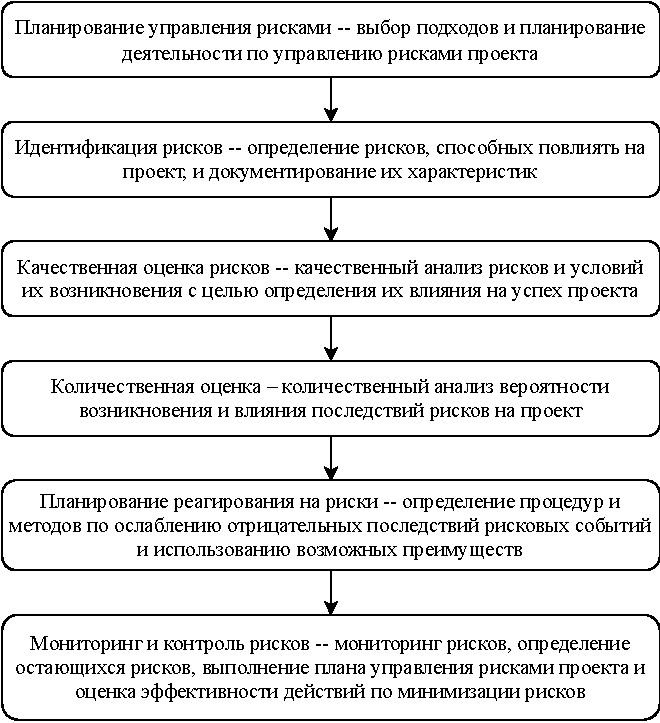
\includegraphics[width=0.7\linewidth]{Diagram-Page-2}
	\caption{Этапы управления рисками проекта}
	\label{fig:diagram-page-2}
\end{figure}

Планирование управления рисками --- процесс принятия решений по применению и планированию управления рисками для конкретного проекта. Этот процесс
может включать в себя решения по организации, кадровому обеспечению процедур
управления рисками проекта, выбор предпочтительной методологии, источников данных
для идентификации риска, временной интервал для анализа ситуации. Важно
спланировать управление рисками, адекватное как уровню и типу риска, так и важности
проекта для организации.

Идентификация рисков --- начальный этап системы мероприятий по управлению рисками, заключающийся в систематическом выявлении рисков, характерных для определенного вида деятельности, и определении их характеристик.

Идентификация сводится к выявлению возможных проблем. 
Под «проблемой» понимают что-либо (событие, объект, человека, идею), что может встать между организацией и ее целями.
Необходимо определить, что пойдет «не так», чтобы затем решить, как это устранить
или обойти.
Идентификация риска – процесс нахождения, составления пе-
речня и описания элементов риска.
Основные элементы риска:
– причины, приводящие к наступлению опасного явления;
– опасные явления (события), оказывающие воздействие на объ-
ект;
– виды воздействия, которые могут привести к изменению со-
стояния объекта;
– последствия, представляющие собой потери из-за воздействия,
и их оценку со стороны субъекта;
– факторы риска, влияющие на вероятность реализации риска
и тяжесть последствий.
